\documentclass[tikz]{standalone}

\usetikzlibrary{positioning, calc}
\usepackage{amsmath,amsfonts}

\begin{document}
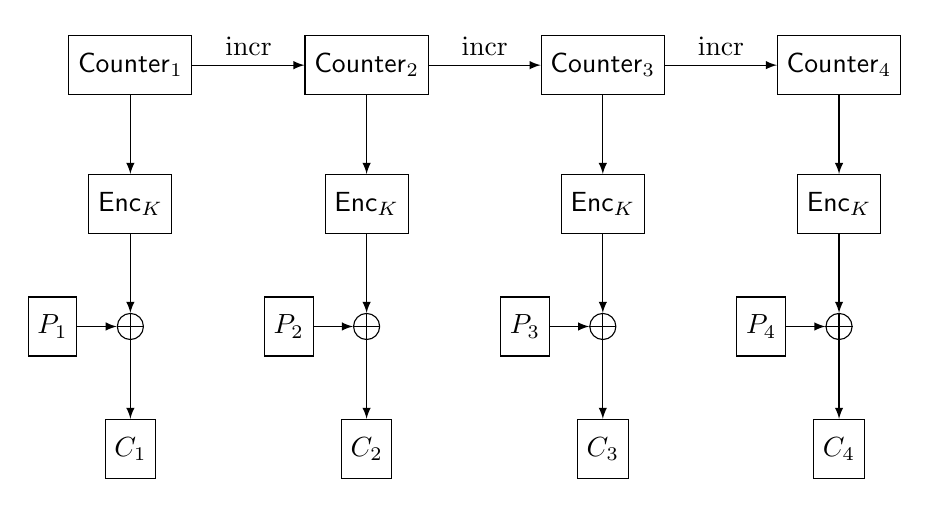
\begin{tikzpicture}
    \foreach \i in {1, 2, 3, 4}
    {
        \node (Ctr\i) at ($\i*(3,0)$) [minimum width=0.75cm, minimum height=0.75cm, draw] {$\mathsf{Counter}_\i$};
        \node (E\i) [below=1cm of Ctr\i, minimum width=0.75cm, minimum height=0.75cm, draw] {$\mathsf{Enc}_K$};
        \node (x\i) [below=1cm of E\i, circle, draw] {};
        \node (P\i) [left=0.5cm of x\i, minimum width=0.5cm, minimum height=0.75cm, draw] {$P_\i$};
        \node (C\i) [below=1cm of x\i, minimum width=0.5cm ,minimum height=0.75cm, draw] {$C_\i$};

        \draw (x\i.north) -- (x\i.south);
        \draw (x\i.west) -- (x\i.east);

        \draw[-latex] (Ctr\i.south) -- (E\i.north);
        \draw[-latex] (E\i.south) -- (x\i.north);
        \draw[-latex] (P\i.east) -- (x\i.west);
        \draw[-latex] (x\i.south) -- (C\i.north);
    }

    \draw[-latex] (Ctr1.east) -- node[above] {incr} (Ctr2.west);
    \draw[-latex] (Ctr2.east) -- node[above] {incr} (Ctr3.west);
    \draw[-latex] (Ctr3.east) -- node[above] {incr} (Ctr4.west);
\end{tikzpicture}
\end{document}